Solving the hyperbolic system \eqref{eq:quasilinear_normal} amounts to construct hyper-surfaces $\Qcb(x_n,t)$, or integral surfaces, given some initial values $\Qcb(x_n,0)$, which is in general difficult.
Nevertheless, the projection of system \eqref{eq:quasilinear_normal} onto the left eigenbasis leads to the set of characteristic equations \cite{Courant}:
\begin{equation}
  \label{eq:charac-equations}
  \Lcb^K \cdot d\Qcb = 0
\end{equation}
where $d\Qcb$ is related to the directional derivative of $\Qcb$ along the $K$th characteristic curve with slope $x_n/t=c_K$ in the $(x_n,t)$ plane.
The integration of the set of ODEs \eqref{eq:charac-equations} yields integral curves that enable, through the method of characteristics, the calculation of self-similar solutions. %, that is, $\Qcb$ is constant along each ray $c_K$.

In what follows, the construction of the integral curves as well as the application of the method of characteristics are developed for general two-dimensional problems as a first result of the present paper.

$\newline$
The projection of the quasilinear form \eqref{eq:quasilinear_normal} onto the left eigenbasis developed in the previous section yields for the fast waves:
\begin{align}
  \label{eq:charac_fr}
  & \rho c_f \vect{l}^1 \cdot d\vect{v} - l^1_i n_j d\sigma_{ij} =0 \: , \quad  x_n/t =  c_f \\
  \label{eq:charac_fl}
  -& \rho c_f \vect{l}^1 \cdot d\vect{v} - l^1_i n_j d\sigma_{ij} =0 \: ,\quad  x_n/t = - c_f
\end{align}
for the slow waves:
\begin{align}
  \label{eq:charac_sr}
  & \rho c_s \vect{l}^2 \cdot d\vect{v} - l^2_i n_j d\sigma_{ij} =0 \: ,\quad  x_n/t =  c_s \\
  \label{eq:charac_sl}
  -& \rho c_s \vect{l}^2 \cdot d\vect{v} - l^2_i n_j d\sigma_{ij} =0\: , \quad  x_n/t = - c_s \end{align}
and at last, for the stationary wave:
\begin{equation}
  \label{eq:charac_contact}
  \alpha_{11}d\sigma_{11} + \alpha_{12}d\sigma_{12} + \alpha_{22}d\sigma_{22}=0 \: ,\quad x_n/t =0
\end{equation}
%Integration of equations \eqref{eq:charac_fr} to \eqref{eq:charac_contact} leads to integral curves through simple waves in which several stress components vary, hence the name combined-stress simple waves \cite{CRISTESCU19591605}.

Analogously to \cite{Clifton}, the method of characteristics is applied by combining equations \eqref{eq:charac_fr} to \eqref{eq:charac_contact}.
\begin{figure}[h!]
  \centering
  \subcaptionbox{Slow simple wave \label{subfig:slowWave}}{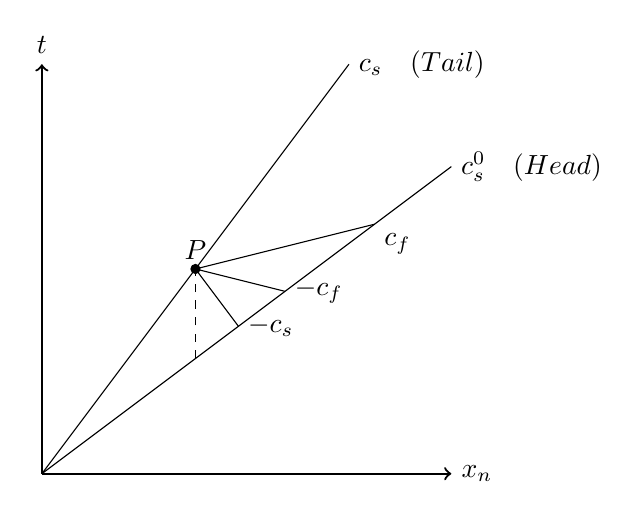
\begin{tikzpicture}[scale=1.3] 
  \newcommand\shift{5.}
  %% Slow
  \draw[thick,->] (0,0) -- (4.,0) node[right] {$x_n$};
  \draw[thick,->] (0,0) -- (0.,4) node[above] {$t$};
  % Slope = 0.75
  \draw (0,0) -- (4,3.) node [right] {$c_s^0 \quad (Head)$};
  % Slope = 4./3.
  \draw (0,0) -- (3.,4.) node [right] {$c_s \quad (Tail)$};

  \fill[black] (1.5,1.5*4./3.) circle (0.05) node [above] {$P$};
  %% Other characteristics
  % stationary
  \draw[dashed] (1.5,0.75*1.5) -- (1.5,1.5*4./3.);
  % fast plus (slope =+-0.25)
  \newcommand\px{1.5}
  \newcommand\py{1.5*4./3.}
  \draw (2.*\py-0.5*\px,1.5*\py-3.*\px/8.) node [below right] {$c_f$}-- (1.5,1.5*4./3.) ;
  % fast minus
  \draw (\py+0.25*\px,0.75*\py+3.*\px/16.) node [right] {$-c_f$} -- (1.5,1.5*4./3.) ;
  % slow minus (slope=-4./3.)
  \draw (12.*\py/25.+16.*\px/25.,9.*\py/25.+36.*\px/75.) node [right] {$-c_s$} -- (1.5,1.5*4./3.) ;
\end{tikzpicture}


%%% Local Variables:
%%% mode: latex
%%% TeX-master: "../../mainManuscript"
%%% End:
} \qquad
  \subcaptionbox{Fast simple wave \label{subfig:fastWave}}{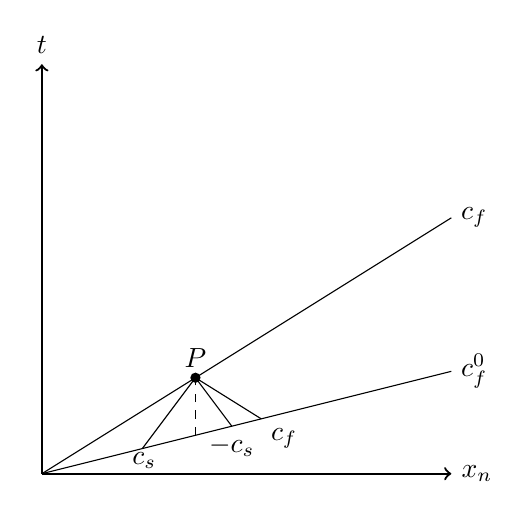
\begin{tikzpicture}[scale=1.3] 
  \newcommand\shift{5.}
  %% Fast
  \draw[thick,->] (0+\shift,0) -- (4.+\shift,0) node[right] {$x_n$};
  \draw[thick,->] (0+\shift,0) -- (0.+\shift,4) node[above] {$t$};
  % Slope = 0.25
  \draw (0+\shift,0) -- (4+\shift,1.) node [right] {$c_f^0$};
  % Slope = 5./8.
  \draw (0+\shift,0) -- (4+\shift,2.5) node [right] {$c_f$};
  
  \fill[black] (1.5+\shift,1.5*5./8.) circle (0.05) node [above] {$P$};
  %% Other characteristics
  \newcommand\pxx{1.5}
  \newcommand\pyy{1.5*5./8.}
  % stationary
  \draw[dashed] (1.5+\shift,1.5/4.) -- (\pxx+\shift,\pyy);
  % fast minus
  \draw (8.*\pyy/7.+5.*\pxx/7.+\shift,2.*\pyy/7.+10.*\pxx/56.) node [below right] {$c_f$}-- (\pxx+\shift,\pyy);
  % slow plus
  \draw (-12.0*\pyy/13.+16.*\pxx/13.+\shift,-3.*\pyy/13.+4.*\pxx/13.) -- (\pxx+\shift,\pyy);
  \node at (-12.0*\pyy/13.+16.*\pxx/13.+\shift+0.02,-3.*\pyy/13.+4.*\pxx/13.-0.12) {$c_s$};
  % slow minus
  \draw (12.0*\pyy/19.+16.*\pxx/19.+\shift,3.*\pyy/19.+4.*\pxx/19.)node [below] {$-c_s$} -- (\pxx+\shift,\pyy);
\end{tikzpicture}


%%% Local Variables:
%%% mode: latex
%%% TeX-master: "../../mainManuscript"
%%% End:
}
  \caption{The method of characteristics through slow and fast simple waves in the $(x_n,t)$ plane.}
  \label{fig:charac_method}
\end{figure}
The approach consists in tracing every characteristic from some downstream point of a wave where the state vector $\Qcb$ is known, to an upstream point where the solution is sought.
Figures \ref{subfig:slowWave} and \ref{subfig:fastWave} schematically illustrate the method for slow and fast simple waves in which the state is known along the head wave and is looked for at the point $P$ lying on the tail wave. 

The right-going slow waves are first looked at by adding equations \eqref{eq:charac_fr} and \eqref{eq:charac_fl}:
\begin{equation}
  l_i^1 n_j d\sigma_{ij}=0
\end{equation}
Given the geometry of the problem, the vector $\vect{n}$ may be reduced to $\vect{e}_1$ or $\vect{e}_2$.
It therefore comes out:
%In particular, for a vector $\vect{n}$ that is restricted to the axis of the $(\vect{e}_1,\vect{e}_2)$ plane, one gets:
\begin{align}
  \label{eq:sigSlow_n=e1}
  & d\sigma_{11} = - \frac{l^1_2}{l_1^1} d\sigma_{12} = \psi^s_{1}d\sigma_{12}  \quad \text{for } \:\vect{n}=\vect{e}_1 \\
  \label{eq:sigSlow_n=e2}
  & d\sigma_{22}=- \frac{l_1^1}{l_2^1}  d\sigma_{12} = \psi^s_{2}d\sigma_{12} \quad \text{for } \:\vect{n}=\vect{e}_2
\end{align}
where $\psi^s_1$ and $\psi^s_2$ are functions of all components of $\tens{\sigma}$. 
Note that the $s$ and $f$ superscripts stand for slow and fast waves respectively in the following.
Next, the characteristic equation related to the contact wave \eqref{eq:charac_contact} reads:
\begin{align}
    \label{eq:sigContact_n=e1}
    & d\sigma_{22} = -\frac{\psi^s_{1}\alpha_{11}+\alpha_{12}}{\alpha_{22}}d\sigma_{12}  \quad \text{for } \:\vect{n}=\vect{e}_1 \\
    \label{eq:sigContact_n=e2}
    & d\sigma_{11}= -\frac{\psi^s_{2}\alpha_{22}+\alpha_{12}}{\alpha_{11}} d\sigma_{12}  \quad \text{for } \:\vect{n}=\vect{e}_2
\end{align}
in which the $\alpha_{ij}$'s are defined in \eqref{eq:null_left_eigen}.
The sets of equations \eqref{eq:sigSlow_n=e1}-\eqref{eq:sigContact_n=e1} and \eqref{eq:sigSlow_n=e2}-\eqref{eq:sigContact_n=e2} show the combined-stress nature of slow simple waves since both longitudinal and transverse components vary, in contrast with elastic waves.
On the other hand, the subtraction of equations \eqref{eq:charac_fr} and \eqref{eq:charac_fl} leads to:
\begin{equation*}
  dv_1 = \psi^s_{1}dv_2 = \frac{1}{\psi^s_2}dv_2
\end{equation*}
which, once combined with equations \eqref{eq:sigSlow_n=e1}-\eqref{eq:sigSlow_n=e2} and introduced in \eqref{eq:charac_sl}, yields after simplifications:
\begin{align}
    \label{eq:vSlow_n=e1}
    & dv_1 = -\frac{d\sigma_{11}}{\rho c_s^2} \quad ;\quad  dv_2 = -\frac{d\sigma_{12}}{\rho c_s^2} \qquad  \text{for } \vect{n}=\vect{e}_1\\
    \label{eq:vSlow_n=e2}
    & dv_1 = -\frac{d\sigma_{12}}{\rho c_s^2} \quad ;\quad  dv_2 = -\frac{d\sigma_{22}}{\rho c_s^2} \qquad  \text{for } \vect{n}=\vect{e}_2
\end{align}

\begin{remark}
  The ODEs through a left-going slow wave result from the combination of equations \eqref{eq:sigSlow_n=e1}-\eqref{eq:sigSlow_n=e2} introduced in \eqref{eq:charac_sr} rather than \eqref{eq:charac_sl}.
  Therefore, the only difference lies in the signs in equations \eqref{eq:vSlow_n=e1} and \eqref{eq:vSlow_n=e2}.
\end{remark}

Similar results are obtained for right-going fast simple waves by using $\vect{l}^2$ instead of $\vect{l}^1$ and $c_f$ rather than $c_s$.
%However, the integral curves involve $\vect{l}^2$ and $c_f$ instead of $\vect{l}^1$ and $c_s$. 
Hence, the evolution in slow and fast waves is governed by the \textit{loading functions}:
\begin{equation}
  \label{eq:loading_func}
  \begin{aligned}
  &\psi^s_{1}=- \left.\frac{l^1_2}{l_1^1}\right\rvert_{\vect{n}=\vect{e}_1} \quad ,\quad \psi^s_{2}=- \left.\frac{l_1^1}{l_2^1}\right\rvert_{\vect{n}=\vect{e}_2} \\
  &\psi^f_1=-\left.\frac{l_2^2}{l_1^2}\right\rvert_{\vect{n}=\vect{e}_1}  \quad ,\quad \psi^f_2=-\left.\frac{l_1^2}{l_2^2}\right\rvert_{\vect{n}=\vect{e}_2}  
  \end{aligned}
\end{equation}
The ODEs satisfied across right-going slow and fast simple waves depending on the direction considered are summarized in table \ref{tab:simpleWavesEquations} for directions $\vect{e}_1$ and $\vect{e}_2$.
\begin{table*}[h!]
  \centering
  \begin{tabular}{cc|ccN}
    \hline
    \multicolumn{2}{c}{Right-going slow wave} \vline& \multicolumn{2}{c}{Right-going fast wave} & \\
    $\vect{n}=\vect{e}_1$ & $\vect{n}=\vect{e}_2$ & $\vect{n}=\vect{e}_1$ & $\vect{n}=\vect{e}_2$&\\
    \hline
    \hline
    $dv_1 = -\frac{d\sigma_{11}}{\rho c_s^2}$ &  $dv_1 = -\frac{d\sigma_{12}}{\rho c_s^2}$ &$dv_1 = -\frac{d\sigma_{11}}{\rho c_f^2}$ &  $dv_1 = -\frac{d\sigma_{12}}{\rho c_f^2}$ &\\ [8pt]
    $dv_2 = -\frac{d\sigma_{12}}{\rho c_s^2}$ & $dv_2 = -\frac{d\sigma_{22}}{\rho c_s^2}$ & $dv_2 = -\frac{d\sigma_{12}}{\rho c_f^2}$ & $dv_2 = -\frac{d\sigma_{22}}{\rho c_f^2}$& \\ [8pt]
    $d\sigma_{11} = \psi^s_{1}d\sigma_{12}$&$d\sigma_{11}= -\frac{\psi^s_{2}\alpha_{22}+\alpha_{12}}{\alpha_{11}} d\sigma_{12}$ &  $d\sigma_{11} = \psi^f_{1}d\sigma_{12}$&$d\sigma_{11}= -\frac{\psi^f_{2}\alpha_{22}+\alpha_{12}}{\alpha_{11}} d\sigma_{12}$ & \\[8pt]
    $d\sigma_{22} = -\frac{\psi^s_{1}\alpha_{11}+\alpha_{12}}{\alpha_{22}}d\sigma_{12}$ & $d\sigma_{22}= \psi^s_{2}d\sigma_{12}$ & $d\sigma_{22} = -\frac{\psi^f_{1}\alpha_{11}+\alpha_{12}}{\alpha_{22}}d\sigma_{12}$ & $d\sigma_{22}= \psi^f_{2}d\sigma_{12}$ & \\[8pt]
    % & & \\
    % & & \\    
    \hline
\end{tabular}
%%% Local Variables:
%%% mode: latex
%%% TeX-master: "../manuscript"
%%% End:

  \caption{Summary of the ODEs satisfied inside right-going slow and fast simple waves.}
  \label{tab:simpleWavesEquations}
\end{table*}

The complete solution is given by the integral curves that result from the integration of those ODEs.
For instance, through a right-going wave in the direction $\vect{e}_1$, the velocity obeys:
\begin{equation}
  \label{eq:integral_example}
  v_1 = v_1^0 - \int_{\tens{\sigma}^0}^{\tens{\sigma}} \frac{d \sigma_{11}}{\rho c^2} \quad ;\quad v_2 = v_2^0 - \int_{\tens{\sigma}^0}^{\tens{\sigma}} \frac{d \sigma_{12}}{\rho c^2}
\end{equation}
where the zero superscript denotes the downstream state.
As emphasized by \textsc{Clifton} \cite{Clifton}, the integrals depend on the loading path and hence, the simple waves involved. 
It is therefore crucial to identify the stress path followed to properly compute integrals \eqref{eq:integral_example}.

% Notice that by considering the elastic stiffness tensor in the derivation of the equations of table \ref{tab:simpleWavesEquations}, one can write the integral curves holding through the elastic waves.
\begin{remark}
  \label{rq:coupled_components}
  Considering the elastic stiffness tensor in the above developments, the equations of elasticity, for which $c_s=c_2$ and $c_f=c_1$, can be derived.
  In that case, one shows that $\psi^s_1=\psi^s_2=0$ and $\psi^f_1=\psi^f_2=\infty$, so that the equations of table \ref{tab:simpleWavesEquations} greatly simplify.
  As a result, jump conditions associated with discontinuous contact waves are written rather than integral curves such as \eqref{eq:integral_example} linked to rarefaction waves, which is due to the path-independent constitutive equations.
  It then turns out that a pressure wave carries jump discontinuities of $\sigma_{nn}$, $\sigma_{tt}$ and $v_n$, where $n$ and $t$ denote normal and transverse components of the propagation direction, whereas a shear wave propagates jump discontinuities in $\sigma_{nt}$ and $v_t$ (see table \ref{tab:elasticityEquations}).
  % This first highlights the difference between plastic simple waves and elastic discontinuities.waves.
\end{remark}
\begin{table*}[h!]
  \centering
  \begin{tabular}{cc|ccN}
    \hline
    \multicolumn{2}{c}{Right-going shear wave} \vline& \multicolumn{2}{c}{Right-going pressure wave} & \\
    $\vect{n}=\vect{e}_1$ & $\vect{n}=\vect{e}_2$ & $\vect{n}=\vect{e}_1$ & $\vect{n}=\vect{e}_2$&\\
    \hline
    \hline
    $\llbracket v_1 \rrbracket = 0 $ &  $\llbracket v_1 \rrbracket= -\frac{\llbracket\sigma_{12} \rrbracket}{\rho c_2^2}$ &$\llbracket v_1 \rrbracket = -\frac{\llbracket \sigma_{11}\rrbracket}{\rho c_1^2}$ &  $\llbracket v_1 \rrbracket = 0 $ &\\ [8pt]
  $\llbracket v_2 \rrbracket= -\frac{\llbracket \sigma_{12} \rrbracket}{\rho c_2^2}$ & $\llbracket v_2 \rrbracket= 0 $ & $\llbracket v_2 \rrbracket= 0$ & $\llbracket v_2 \rrbracket= -\frac{\llbracket \sigma_{22} \rrbracket}{\rho c_1^2}$& \\ [8pt]
    $\llbracket \sigma_{11} \rrbracket= 0$ & $\llbracket \sigma_{11} \rrbracket=0 $ &  $\llbracket \sigma_{12} \rrbracket= 0 $&$\llbracket \sigma_{12} \rrbracket= 0$ & \\[8pt]
    $\llbracket \sigma_{22} \rrbracket= 0 $ & $\llbracket \sigma_{22} \rrbracket= 0 $ & $\llbracket \sigma_{22} \rrbracket= -\frac{\alpha_{11}}{\alpha_{22}}\llbracket \sigma_{11}\rrbracket$ & $\llbracket \sigma_{11} \rrbracket= -\frac{\alpha_{22}}{\alpha_{11}} \llbracket \sigma_{22} \rrbracket$ & \\[8pt]

  \hline
\end{tabular}
%%% Local Variables:
%%% mode: latex
%%% TeX-master: "../manuscript"
%%% End:

  \caption{Summary of the jump conditions across right-going elastic shear and pressure waves.}
  \label{tab:elasticityEquations}
\end{table*}


% Aij = nk Hikjl nl:
% A12 = n1^2 H1121 + n2^2 H1222
% A11 = n1^2 H1111 + n2^2 H1212
% A22 = n1^2 H2121 + n2^2 H2222
% n1: A11= H1111 ; A12 = 0 ; A22 = H2121 ; om2 = mu ; l2 = [0 , lam + mu] ; om1 = lamb + 2mu ; l1 = [ -lamb - mu , 0 ] => psi^s_1 = 0 ; psi^f_2 = infty
% n2: A11= H1212 ; A12 = 0 ; A22 = H2222 ; om2 = mu ; l2 = [lam + mu , 0] ; om1 = lamb + 2mu ; l1 = [ 0 , -lamb-mu ] => psi^s_2 = 0 ; psi^f_2 = infty


%%% Local Variables:
%%% mode: latex
%%% TeX-master: "manuscript"
%%% End:
